\section{Conclusioni}
Nel trarre le conclusioni riguardo questo lavoro, appare opportuno scindere esplicitamente i due aspetti analizzati: l'applicabilit\`a ed efficacia teorica del processo di acquisizione ed elaborazione e l'implementazione specifica presa in esame.
\subsection{Efficacia del modello teorico}
Il modello teorico su cui si basa l'approccio studiato sembra essere promettente. Esso infatti permette l'archiviazione in formato digitale di materiale audio, spesse volte unico, per mezzo di una procedura rigorosa e ben documentata che richiede all'utente solamente la disponibilit\`a di uno scanner flatbed ampiamente disponibile nei comuni canali commerciali., rendendo di fatto accessibile al grande pubblico la conservazione di materiale d'epoca.

Nonostante l'apparenza iniziale, tuttavia, analizzando nel dettaglio il processo sono state scoperte diverse insidie (quali per esempio la necessaria determinazione del punto di illuminazione ottimale e la procedura intrinsecamente euristica di rilevazione delle tracce) che, di fatto, limitano la fruibilit\`a di questo approccio ad un'utenza con un grado di esperienza medio alto. 

Importante \`e inoltre notare che la necessit\`a di immagini ad alta risoluzione e il processo di elaborazione matriciale necessario all'estrapolazione dell'informazione sonora, richiedono, di fatto, una potenza computazionale non indifferente, limitando ulteriormente la fruibilit\`a di un possibile sistema basato su questo modello teorico ai possessori di architetture hardware di alta fascia.

\subsection{Efficacia dell'implementazione}
L'implementazione fornita dal gruppo della Princeton University \`e risultata essere, a differenza di quanto dichiarato dagli sviluppatori, in uno stadio fortemente prototipale.

I problemi evidenziati nella trattazione precedente rendono il progetto interessante unicamente dal punto di vista accademico e non rendono certo auspicabile una sua diffusione su ampia scala.\\
\`E inoltre interessante notare come i risultati ottenuti in fase di testing del progetto si discostino di molto dai risultati dichiarati dagli sviluppatori. Il file audio ottenuto risulta infatti, anche sotto l'aspetto dell'analisi spettrale, privo di qualunque informazione sonora
\begin{figure}[h!t]
\begin{center}
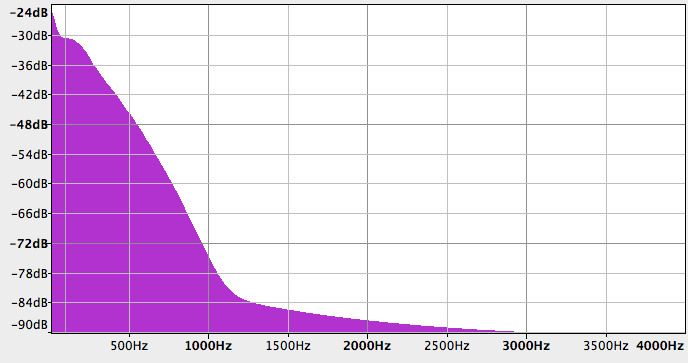
\includegraphics[scale=0.35]{./img/freq-domain.png}
\caption{Spettro del segnale estratto}
\end{center}
\end{figure}
 e di conseguenza inutilizzabile anche nell'eventualit\`a di sofisticati filtri di rimozione del rumore e sound enhancement.

\subsection{Sviluppi futuri}
I risultati ottenuti e le considerazioni fin'ora descritte portano a concludere che il processo di scansione - acquisizione - elaborazione non sia la strada migliore da seguire per portare all'attenzione del pubblico un sistema di digitalizzazione di materiale audio contenuto in dischi in gommalacca.

Altri approcci pi\`u sofisticati che prevedano l'utilizzo di strumenti pi\`u avanzati (quali microscopi o interferometri) potrebbero in'ultima anlisi permettere di acquisire informazione sonora di sufficiente qualit\`a al prezzo, per\`o di limitare l'utilizzo di tali sistemi a soli centri specializzati con le capacit\`a economiche necessarie all'acquisto dei succitati dispositivi e dotati di personale specializzato nell'uso di questi ultimi.
